%%%%%%%%%%%%%%%%%%%%%%%%%%%%%%%%%%%%%%%%%%%%%%%%%%%%%%%%%%%%%%%%%%
%%  ~ Trabajo de Fin de Grado - Universidad de Vigo (ESEI) ~    %%
%% Autor: Diego Enrique Fontán Lorenzo                          %%
%% Tutor: Miguel Ramón Díaz-Cacho Medina                        %%
%% Convocatoria: Julio 2020/21                                  %%
%% Título: Framework de automatización de auditorías Red Team   %%
%%%%%%%%%%%%%%%%%%%%%%%%%%%%%%%%%%%%%%%%%%%%%%%%%%%%%%%%%%%%%%%%%%

%%%%%%%%%%%%%%%%%%%%%%%%%%%%%
%% Tests
%%%%%%%%%%%%%%%%%%%%%%%%%%%%%

\chapter{Pruebas realizadas} \label{cap:tests}

En este capítulo se detallan algunas de las pruebas llevadas a cabo durante la realización del proyecto, con el objetivo de asegurar el funcionamiento del programa, sus posibles aplicaciones en entornos reales y la correcta implementación de los requisitos descritos en el apartado \ref{cap:requirements}.\n

%%%%%%%%%%%%%%%%%%%%%%%%%%%%%
%% Disponibility
%%%%%%%%%%%%%%%%%%%%%%%%%%%%%

\section{Pruebas de disponibilidad e integridad} \label{sec:disptest}

El proyecto debe contar con la capacidad de garantizar que tanto el sistema como los datos van a estar disponibles al usuario en todo momento.\sn

Con el fin de evidenciar este aspecto, se han realizado \textbf{pruebas de estrés} y \textbf{de rendimiento}.\sn

\large
\textbf{Pruebas de estrés y rendimiento}\sn
\normalsize

Consisten en medir la capacidad del sistema en función a la carga de trabajo y sus tiempos de respuesta. Este tipo de pruebas \textbf{dependen de las especificaciones del sistema operativo anfitrión}, sus procesos y la calidad de la conexión a Internet\footnote{Pruebas realizadas sobre Ubuntu 20.04 con 8Gb de RAM, 2Gb de \textit{swap}, procesador Intel Core-i7 8th Gen y conexión por wifi (72Mbps descarga/89Mbps subida).}.\sn

Respecto al rendimiento, se ha realizado un \textit{benchmarking} mediante el uso de la herramienta \textbf{\textit{go-wrk}}\footnote{\url{https://github.com/tsliwowicz/go-wrk}}. A pesar de que \textit{Golang} cuenta con herramientas nativas de \textit{profiling}, no ofrece un buen soporte para realizar este tipo de pruebas sobre servicios \textit{HTTP}.\sn

Se han realizado tres pruebas de estrés en las que se pide a la \textit{\textbf{API}} que interaccione con una, dos y cuatrocientas páginas web reales, respectivamente. La capacidad y los tiempos de respuesta medidos durante 10 segundos son los mostrados en las figuras \ref{fig:benchAPI1URL} y \ref{fig:benchAPI2URL}. La última prueba no ha pasado el control debido a que una única petición a cuatrocientas \textit{URLs} simultáneas tarda aproximadamente medio minuto (\textit{Figs. \ref{fig:benchAPI400URL} y \ref{fig:API400URL}}).\sn

\begin{figure}[H]
    \centering
    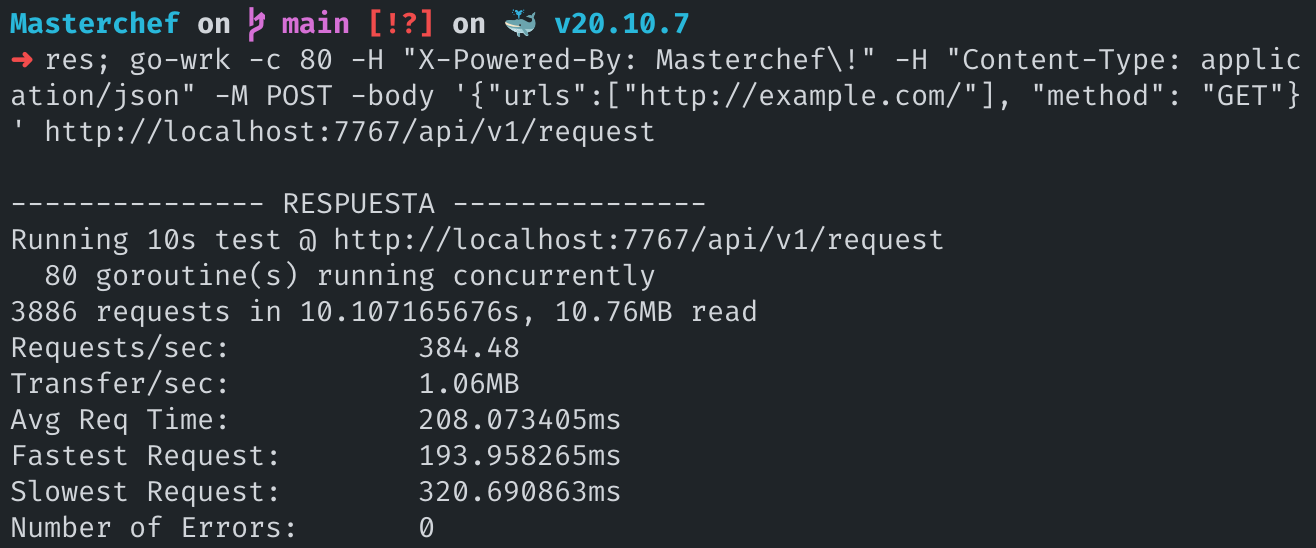
\includegraphics[width=13cm]{img/tables/28_Bench-API-1URL.png}
    \caption{\textit{Benchmark}: 3886 peticiones a 1 \textit{URL}. ~208ms/respuesta. 0 errores.}
    \label{fig:benchAPI1URL}
\end{figure}

\begin{figure}[H]
    \centering
    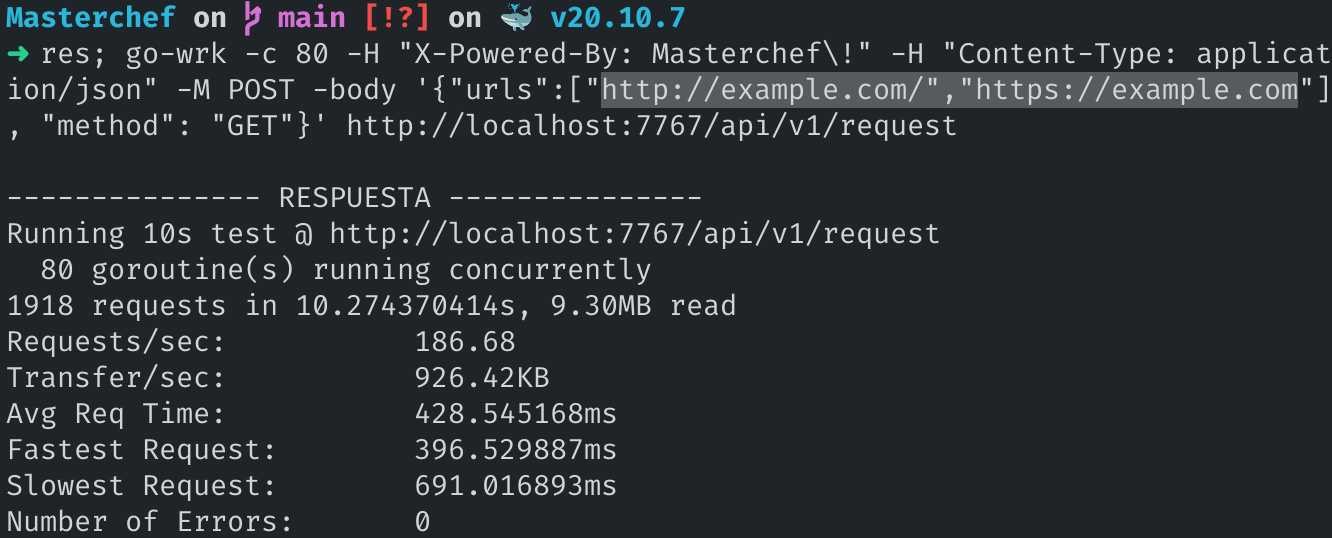
\includegraphics[width=13cm]{img/tables/29_Bench-API-2URL.png}
    \caption{\textit{Benchmark}: 1918 peticiones a 2 \textit{URLs} simultáneas. ~428ms/respuesta. 0 errores.}
    \label{fig:benchAPI2URL}
\end{figure}

\begin{figure}[H]
    \centering
    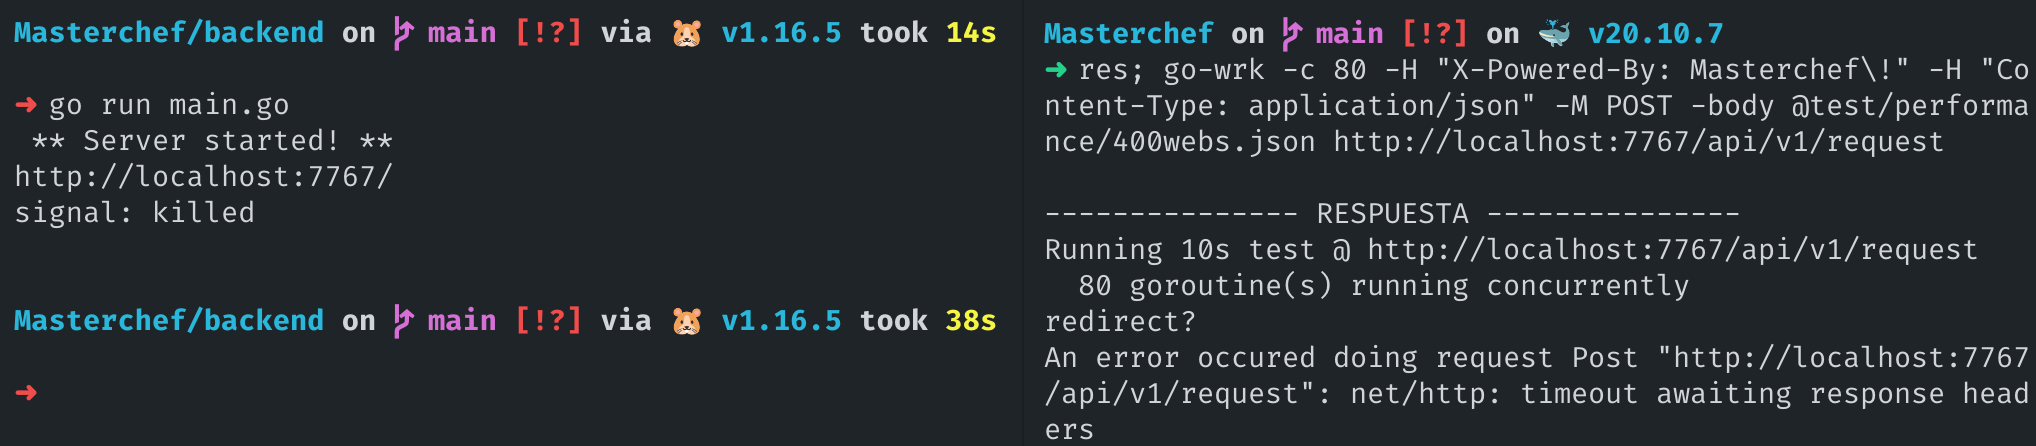
\includegraphics[width=15cm]{img/tables/31_Bench-API-400URL.png}
    \caption{\textit{Benchmark}: Peticiones a 400 \textit{URLs} simultáneas. Prueba de estrés fallida.}
    \label{fig:benchAPI400URL}
\end{figure}

\begin{figure}[H]
    \centering
    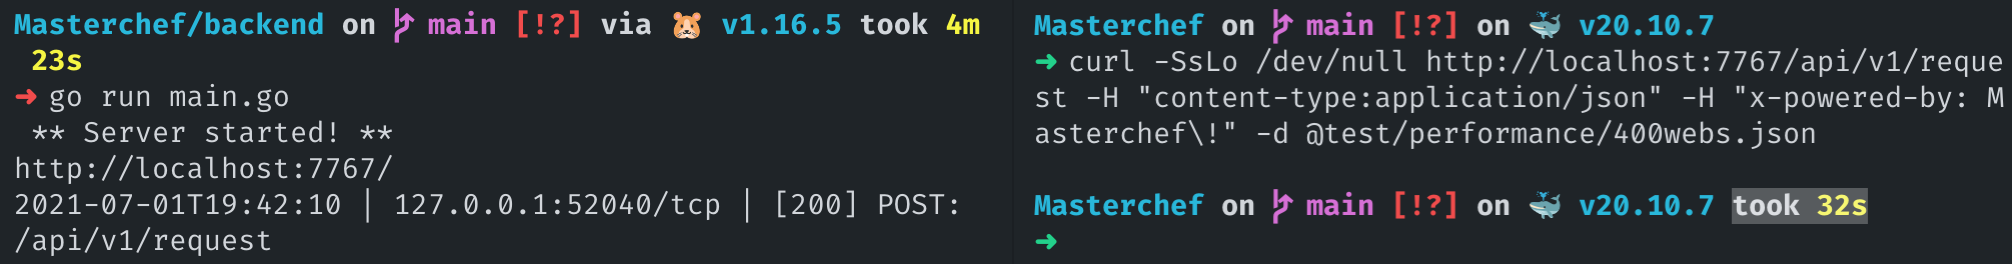
\includegraphics[width=15cm]{img/tables/32_Request-API-400URL.png}
    \caption{\textit{Test}: Petición a 400 \textit{URLs} simultáneas. ~32s/respuesta. 0 errores.}
    \label{fig:API400URL}
\end{figure}

%%%%%%%%%%%%%%%%%%%%%%%%%%%%%
%% Functionality
%%%%%%%%%%%%%%%%%%%%%%%%%%%%%

\section{Pruebas sobre la funcionalidad} \label{sec:functest}

Para comprobar la correcta funcionalidad del sistema, se han ejecutado varios tipos de flujos de datos. Estas pruebas garantizan que se cumplen los requisitos funcionales descritos en el apartado \ref{sub:funcrequirements}.\sn

La figura \ref{fig:multiplerecipe} muestra la capacidad de poder crear conjuntos de tareas independientes entre sí, así como la posibilidad de definir múltiples objetivos.\sn

\begin{figure}[H]
    \centering
    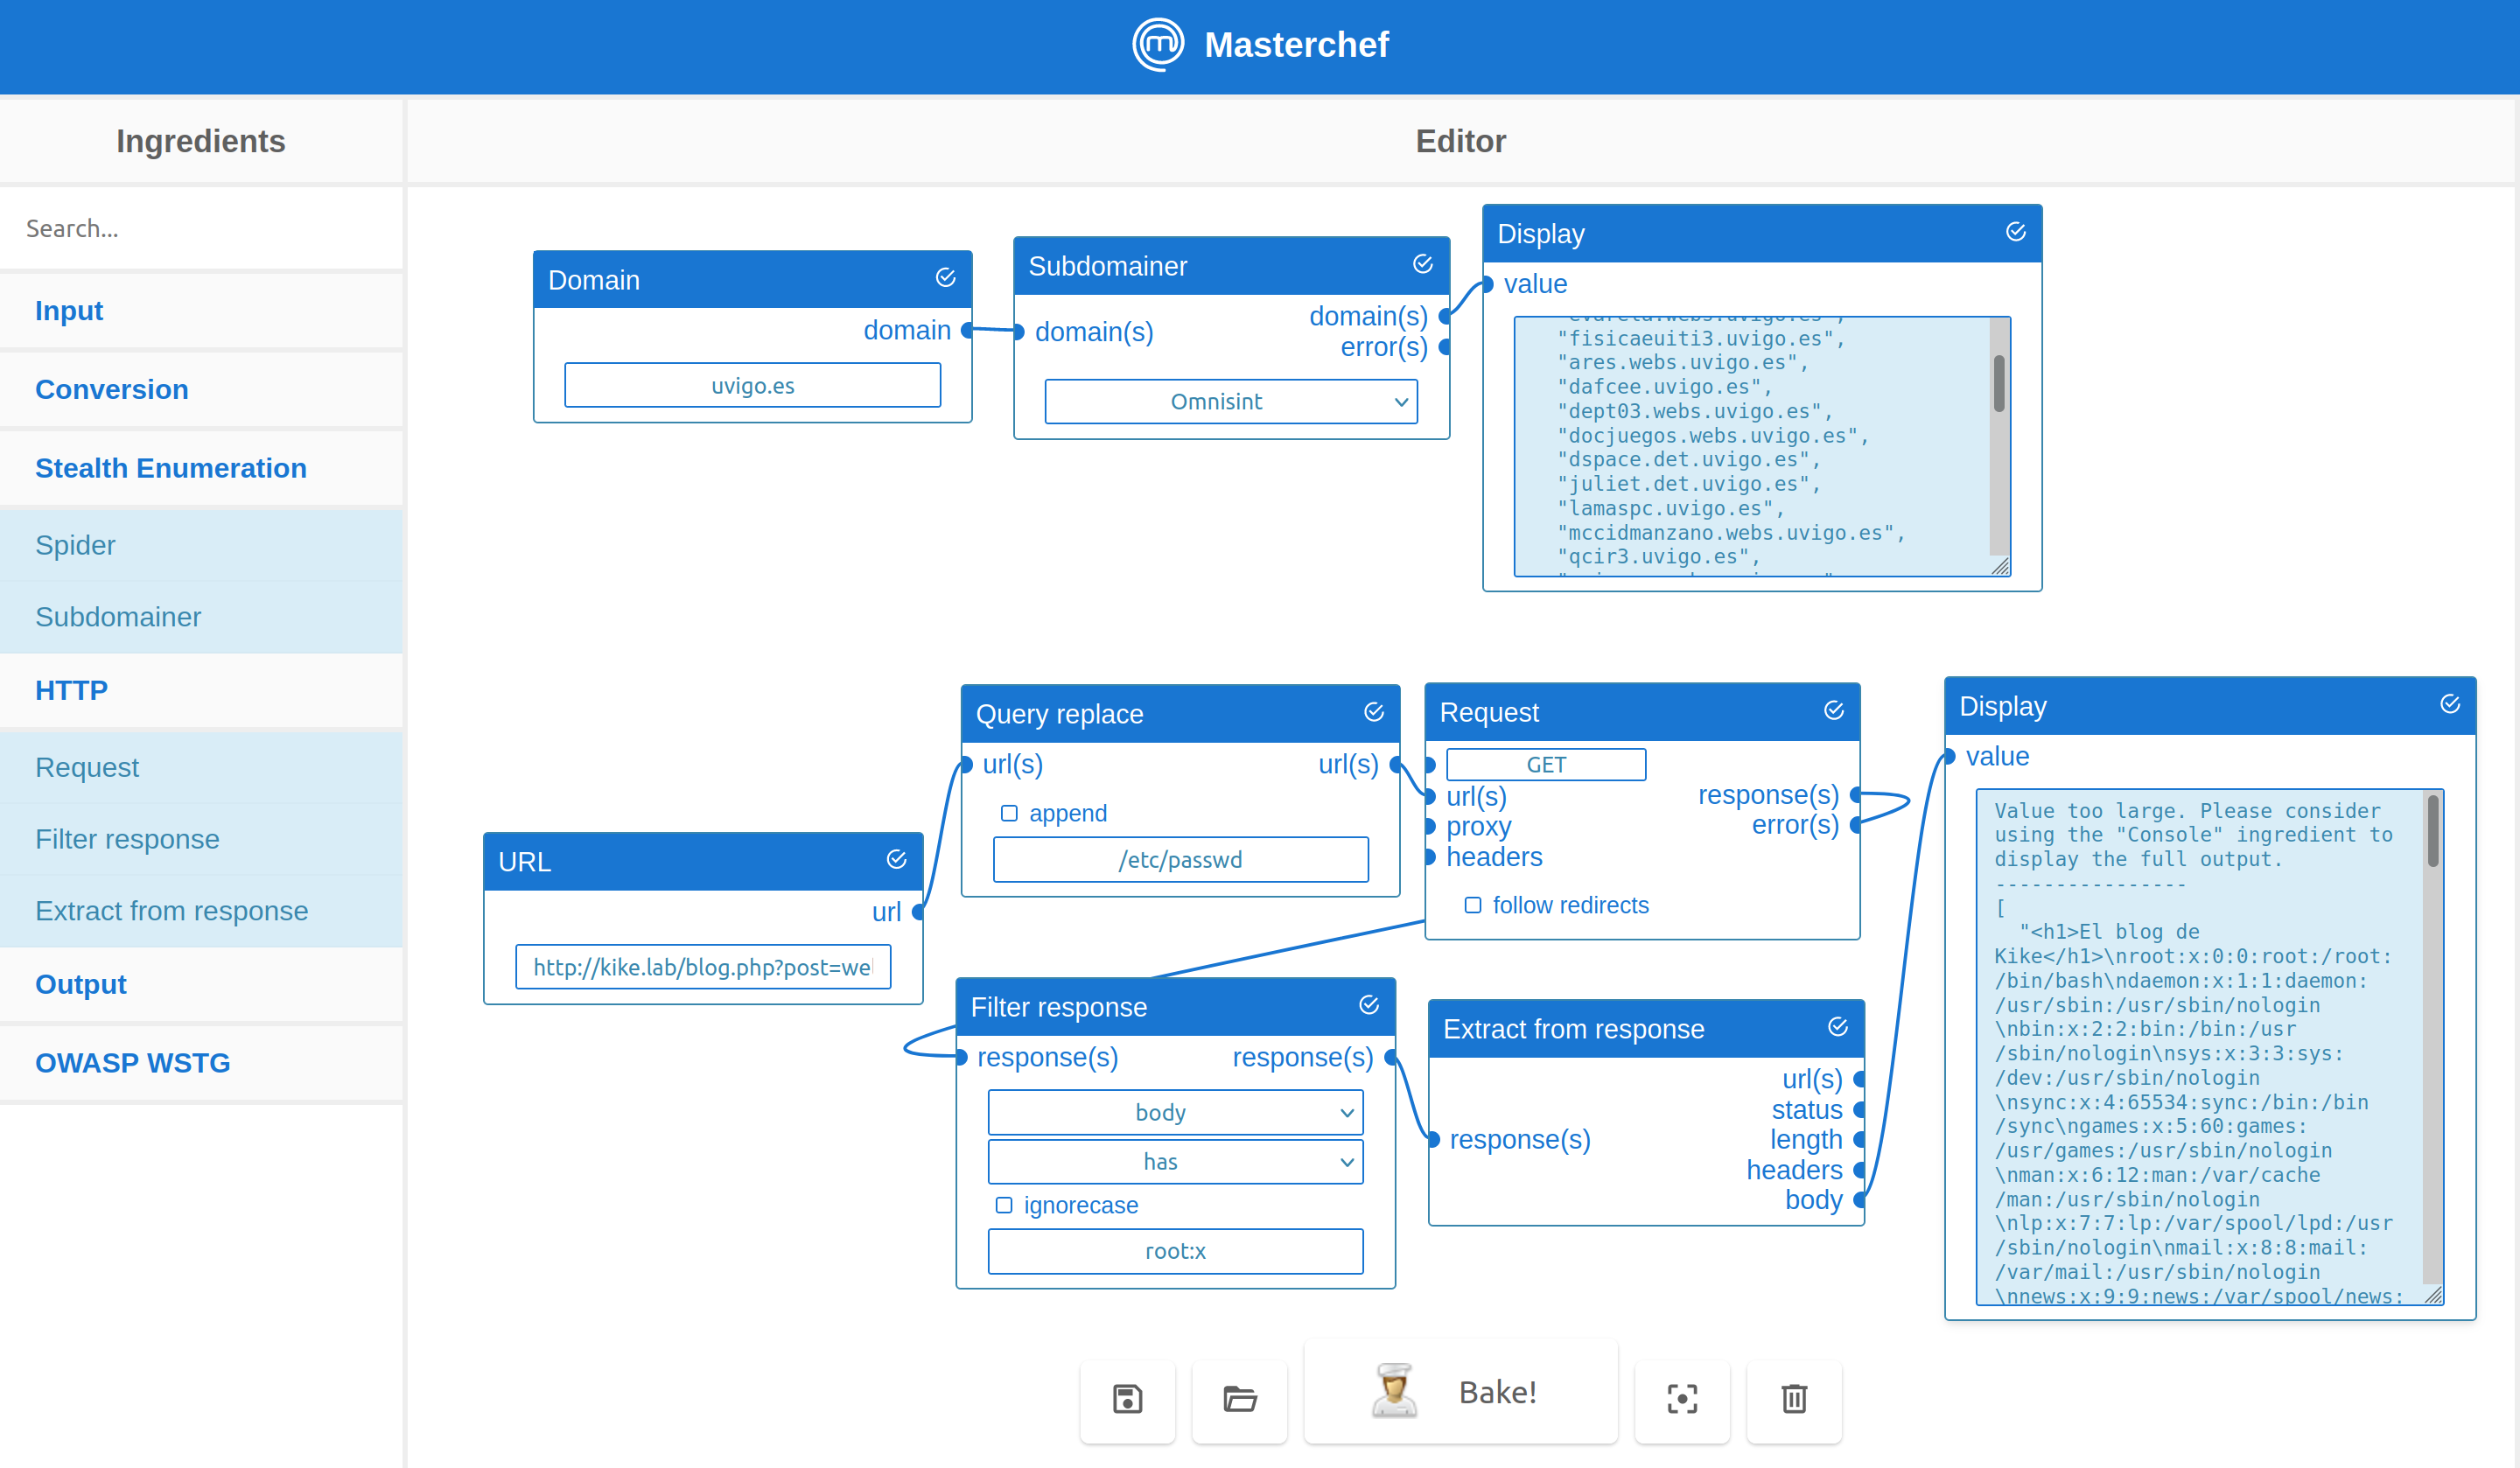
\includegraphics[width=13cm]{img/tables/33_Recipe-Multiple.png}
    \caption{Flujos independientes: Reconocimiento (arriba) y vulnerabilidad (abajo).}
    \label{fig:multiplerecipe}
\end{figure}

Además, en la figura \ref{fig:owasprecipe} se muestra cómo es posible realizar controles propios de una auditoría (ver Anexo \ref{anx:owasp}) a partir de un activo.\sn

\begin{figure}[H]
    \centering
    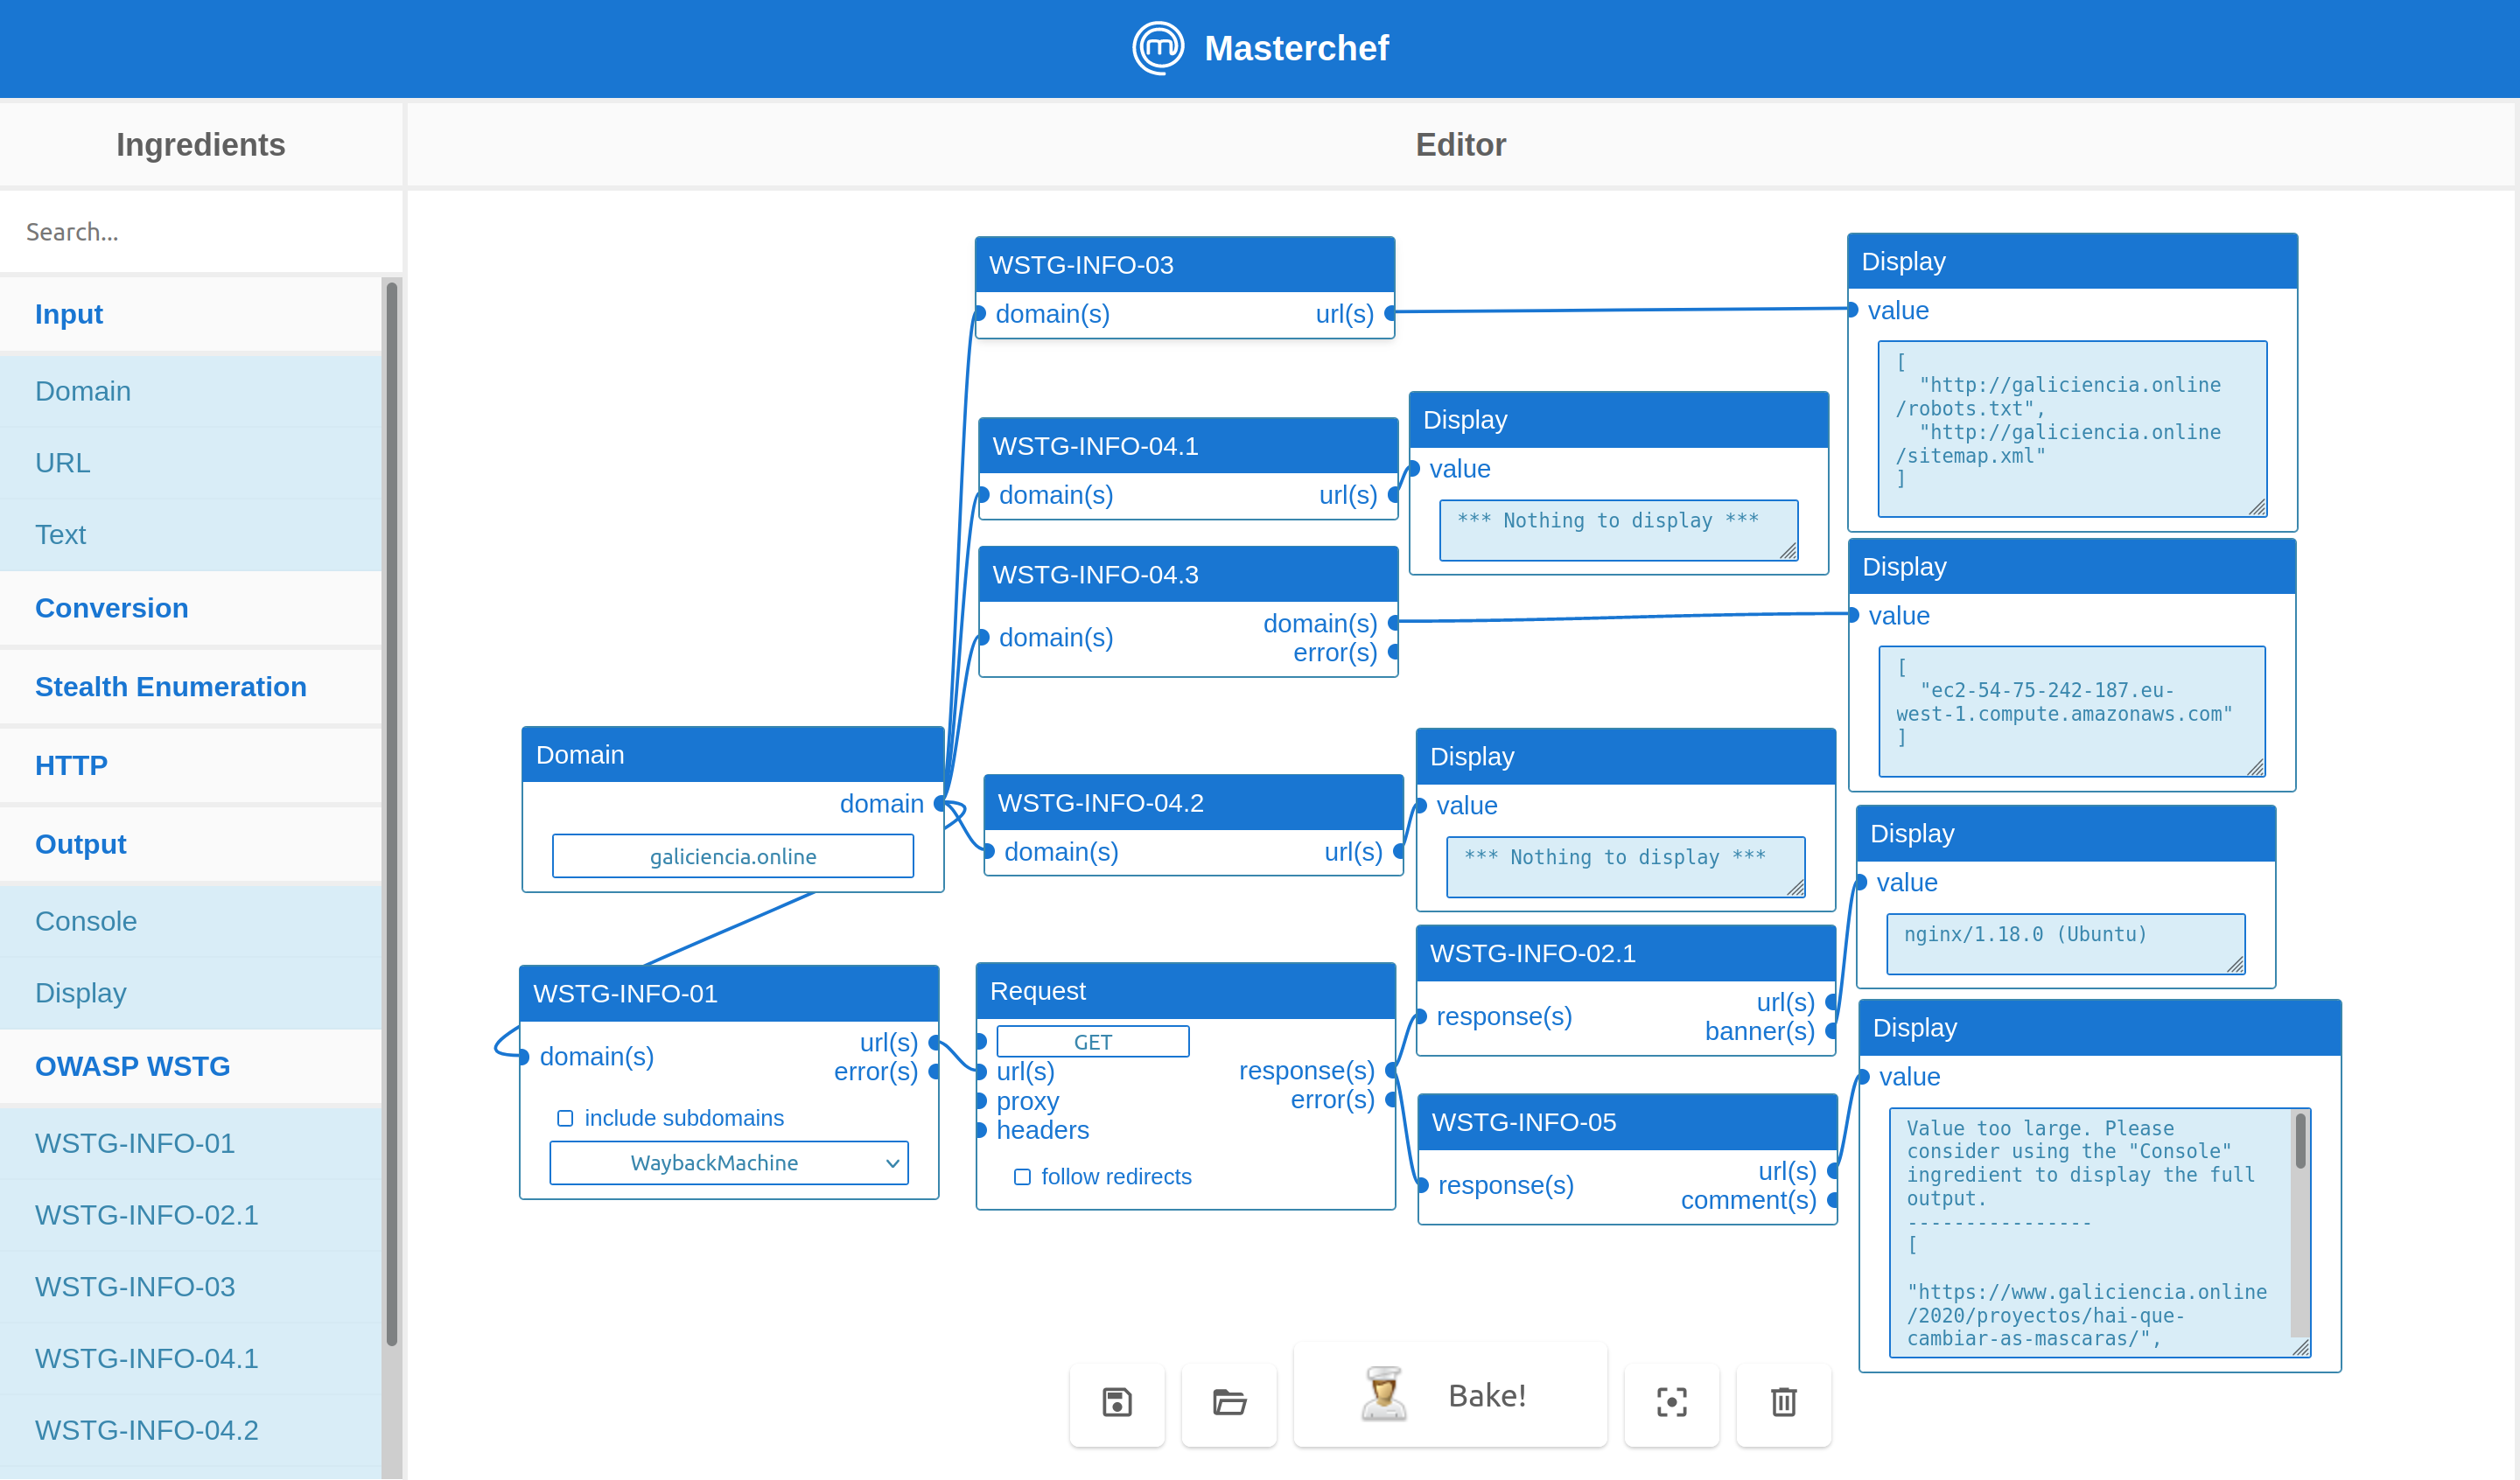
\includegraphics[width=13cm]{img/tables/34_Recipe-WSTG.png}
    \caption{Ejemplo de controles pertenecientes a \textit{OWASP WSTG-INFO}.}
    \label{fig:owasprecipe}
\end{figure}

%%%%%%%%%%%%%%%%%%%%%%%%%%%%%
%% Security
%%%%%%%%%%%%%%%%%%%%%%%%%%%%%

\section{Pruebas de seguridad} \label{sec:securitytest}

Por último, se han realizado pruebas de seguridad para garantizar la ausencia de vectores de ataques que puedan poner en peligro el sistema.\sn

Relativo al editor de nodos, las pruebas constan de la correcta gestión de errores, como bucles infinitos, que podrían provocar una sobrecarga de la \textit{CPU} \fig{reciperr}.

\begin{figure}[H]
    \centering
    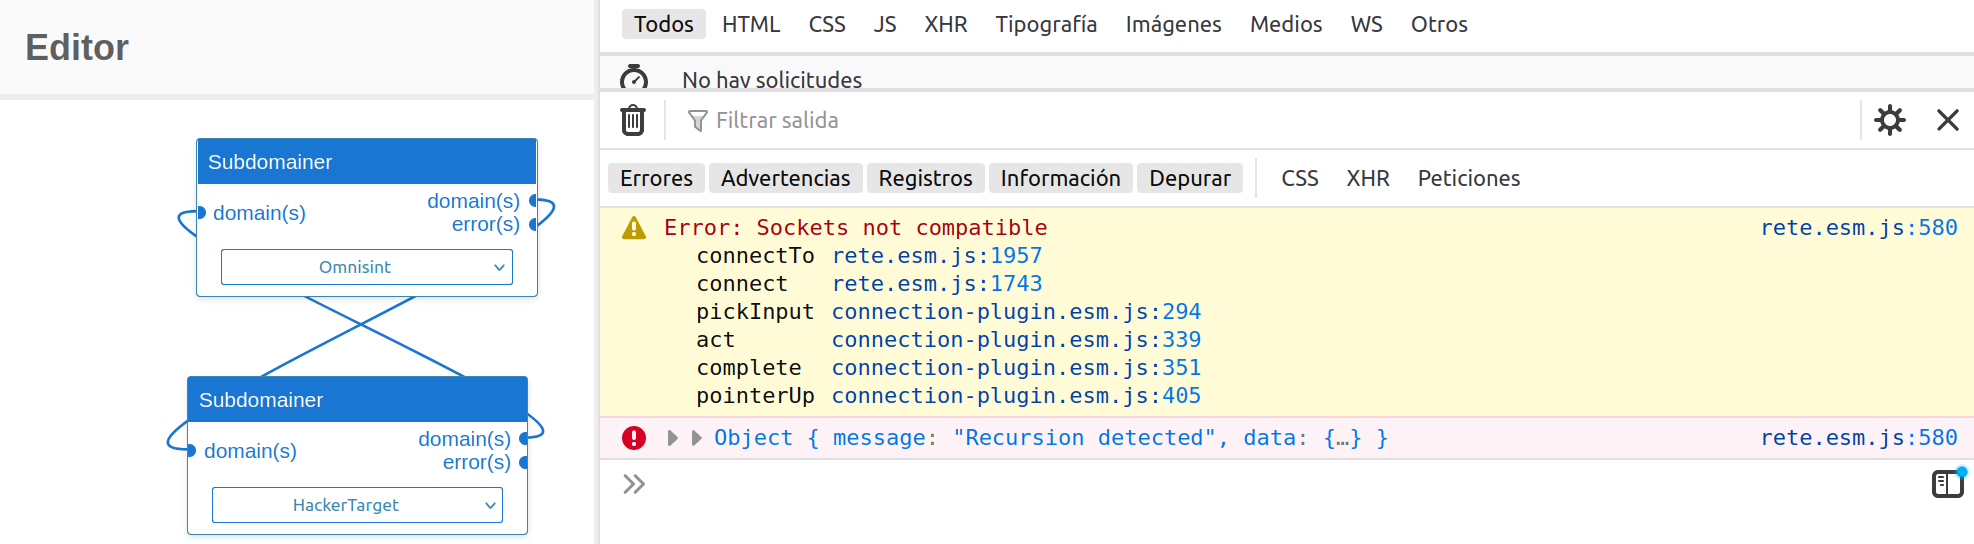
\includegraphics[width=14cm]{img/tables/35_Recipe-Errors.png}
    \caption{Manejo de errores: Conexiones incompatibles y bucles infinitos.}
    \label{fig:reciperr}
\end{figure}

Por otro lado, se han implementado medidas de seguridad para evitar los ataques web más comunes, como \textit{XSS} o \textit{Clickjacking}, mediante el uso de etiquetas \textit{span}\footnote{Las etiquetas \textit{span} no permiten la renderización de código \textit{HTML}} y cabeceras de seguridad \fig{securityrecipe}.\sn

\begin{figure}[H]
    \centering
    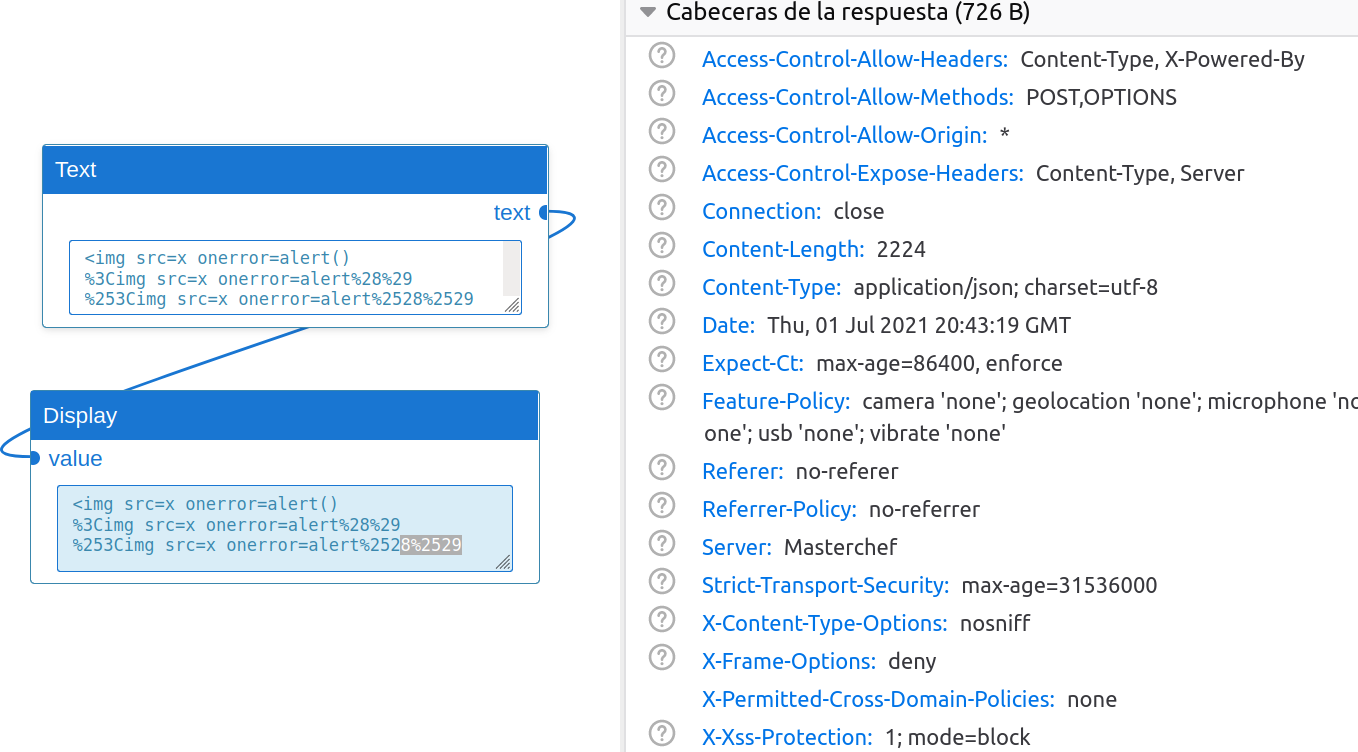
\includegraphics[width=14cm]{img/tables/36_Security.png}
    \caption{Cabeceras de seguridad y pruebas contra \textit{XSS}.}
    \label{fig:securityrecipe}
\end{figure}

Por último, el servidor se interrumpe cuando detecta peticiones más grandes de lo normal contra la \textit{API} \fig{benchAPI400URL}. Esto no se trata de una medida de seguridad, sino de una gestión de errores temporal que tendrá que ser reemplazada por medidas reales, como la segmentación de las peticiones o la implementación de listas negras.\n